\documentclass[12pt]{article}
\usepackage{float}
\usepackage{graphicx}
\usepackage{fontspec}
\usepackage{titlesec}
\usepackage{setspace}
\usepackage[style=numeric,backend=biber,sorting=none]{biblatex}
\usepackage[a4paper, total={6in, 8in}, margin=0.5in]{geometry}
\addbibresource{ref.bib}

%%%%%%%% FORMAT
\singlespacing
\setmainfont{Arial}

\titleformat*{\section}{\normalsize\bfseries}
\titleformat*{\subsection}{\normalsize\bfseries}

\pagenumbering{gobble} % Suppress page number

% \titlespacing\section{0pt}{12pt plus 4pt minus 2pt}{0pt plus 2pt minus 2pt}
% \titlespacing\subsection{0pt}{12pt plus 4pt minus 2pt}{0pt plus 2pt minus 2pt}
% \titlespacing\subsubsection{0pt}{12pt plus 4pt minus 2pt}{0pt plus 2pt minus 2pt}


\begin{document}
  
%%%%%%%%% TITLE  
\title{\large The important role of pharmacokinetics in the drug research and development \vspace{-2em}}
% \author{\large Yujia Shi\vspace{-1em}}
\date{\vspace{-2.5em}}
\maketitle

%%%%%%%%% BODY TEXT
\section{INTROUDCTION}
Pharmacokinetics originates from two Greek words: 'pharmakon' and 'kinetikos', two of which respectively mean the drug and the motion or something else relevant to the motion. Pharmacokinetic is the branch of pharmacology study, aiming at studying the time-courses and metabolite kinetics of substances, such as pharmaceutical, food additives as well as drugs that go through a living organism of whole blood, plasma, or serum. By measuring an adequate amount of time of drug concentrations in the format of biological fluid, like urine, blood, plasma, serum, which open up a possibility to look at the information of invisible drug within different body chamber. Therefore, including Pharmacokinetic study into the routine workflow of pharmacological assessments will beneficial for academic and clinical research to provide additional fundamental research support and manpower for drug discovery and development,  to assist in selecting and designing ideal drug candidates for patients to receive safe and effective therapies. \medskip

Pharmacokinetic is a scientific discipline in which multiple methodologies or mathematical approaches have been used to revealing the pharmacokinetic basics of drugs. Pharmacokinetic can be roughly divided into four classes of study, in terms of a drug being absorbed, distributed, metabolized, and excreted through the body, we often refer to the above processes as the ADEM scheme. Although the golden standard of the ADEM scheme is well enough for us to determine and predict the drug concentrations with the body over time, sometimes, additional studies should be included, as they playing a critical in drug research and further development. For example, liberation, meaning the process of release of drugs from the administered form into an organism body, serves an essential role in maintaining the bio-physiological equilibrium, the velocity of which also significantly determines the pharmacological deposition within the body, the release types can be falls into three-way: immediate, delayed, extended; while other two aspects we also need to take into considerations, response ane toxic effects both are two key reasons for drug discovery failure. Thus, instead of only referring to the PK form of the drug in ADEM studies, investing time and effort looking into more liberation, response, and toxicity, the understanding of the Pharmacokinetic behavior of the drug candidates can be improved. We will further elaborate on the ADEM scheme below(\textbf{See figure 1})\medskip




\subsection{Absorption}
Absorption is a term, describing the course of unmetabolized drug substances entering into the body circulation system. Drug substances can be absorbed through crossing semipermeable cell membranes to reach the target of the site by passive diffusion, Facilitated passive diffusion, Active transport, and Pinocytosis. The greatest site for drug absorption and distribution is the gastrointestinal tract, however, it may be impacted by multiple factors include (i)Drug formulation, the drug is designed into tablets, capsules, suppository, or solution. (ii)route of administration (e.g. buccal, oral, rectal, intravenous, topical, or pulmonary absorption) Comparing with various other administration routes of drug delivery, the oral route of drug administration is a high degree of acceptance in society, as it is the safety, economical and pain avoidance way to take various types of medicine.


\subsection{Distribution}
Drug distribution is one of the processes incorporated in Pharmacokinetic, it is an active and complex process that goes with other pharmacokinetic processes such as drug metabolism and excretion. Understand the mechanism of drug distribution is important in evaluating the dose of the drug will take effect for the target organ and designing the loading dose of the drug. After drug travel into our body, it will be generally distributed throughout in the fluid(e.g. blood, semen, saliva) and various tissue(e.g. bone, blood, and lymph) in the body. Drug distribution is a two-stage process, in the initial phase, the drug will be naturally transported to highly vascular organs such as the liver, kidney, and brain, they will receive most of the drug; while in the second phase, the phenomenon of the redistribution for some drugs to the adipose tissue may occur in this stage. The movement of the drug may be subjected to several factors such as Tissue binding, Regional pH, Cell membrane permeability, and so on, so the drug distribution is usually uneven. When the rate of entry and exit of a drug in the blood and tissue is equal, at a time point, the drug will achieve a distribution equilibrium and the concentration of the drug in the blood plasma will echo the concentration of the drug in tissues and extracellular fluids.


\subsection{Metabolism}
Drug metabolism is the term to describe the process of biotransformation reaction(e.g.Oxidation, Hydrolysis, xenobiotic) of the chemical substance to in living organisms. The primary site for drug metabolism is in the liver, as the particularized enzymatic systems naturally accumulated in this site, to speed up the drug metabolism so that the drug substance can be easily eliminated from the body. Several factors will greatly influence the rate of drug metabolisms such as Physiological(e.g. gender, age, individual variation)and pathological(e.g chronic disorders) factors, thus the drug metabolism rate is varied among people. Due to the difference in drug metabolism, this might affect the efficiency and poisonousness of the drug for patients. For example, for patients with high metabolism rates that impede drug substance to fully exert their therapeutic effect, a drug substance is rapidly excreted from the body before the therapeutic concentration in the blood and tissue is reached. In other patients, due to low metabolism rates, the drug substance will not be cleared out from the body in the shortest of time, usually, they will be concentrated in the bloodstream which poses a higher potential for adverse effects. Drug metabolism consists of two-phase: Phase I is Non-synthetic reactions, such as oxidation, reduction, hydrolysis, formation, or modification, all of these reactions will increase the solubility of drug substances, facilitating them excreted rapidly via the kidneys. Besides, the above reaction process will be catalyzed by a specialized group of an enzymatic system that plays an indispensable role in drug metabolism. Phase II is synthetic reactions, the activated metabolites produced in Phase I will be conjugated with endogenous species such as glutathione (GSH), sulfate, glycine, or glucuronic acid. The weight of products from the conjugation process has been an increase and will be less active than the metabolites formed in Phase I.
\subsection{Excretion}
The last process involved in pharmacokinetics is called Excretion, which is the term to describe the process of removal of pharmaceutical substances from the body. Most of the excretion process will occur in the kidneys.



\medskip
\section{Pharmacokinetics and drug development}
The process for new drug development consists of two different stages: discovery and development. According to the information from the Tufts Center for the Study of Drug Development, three main reasons hinder the development of a new drug: safety, efficiency, and acceptable ADME properties.
Due to a lack of safety, efficiency, and understanding in Pharmacokinetic and bioavailability, making researchers unable to conduct the drug discovery process. Things have been greatly improved in 2000, especially in Pharmacokinetic, with continued hard work and investment to overcome our limited understanding in Pharmacokinetic and bioavailability, the failure rate of drug development has declined dramatically from 40\% to 10\%. Thus, it is possible to perform a cost-effective and efficient drug discovery process in drug candidate's design and selection, when a profound and better understanding of kinetics behavior of the drug candidates. This begs the questions that what made Pharmacokinetic become an indispensable component to the drug discovery process and facilitate unpromising new drugs. The concept of Pharmacokinetic was established in 1960 and become the routine workflow for drug discovery projects in animals, however,
when it comes to how to apply the Pharmacokinetic study in design and explanation of the next drug’s development in human, there still have some gaps ahead of us. It was not until the emergence of new computational technologies that facilitate the process of estimating human pharmacokinetic, therapeutic dose, and gathering the information of absorption, distribution, metabolism, and excretion properties as rapidly and cost-efficient as possible. Several approaches currently can be used to predict human Pharmacokinetic, including from the silicon methods through in vitro-in vivo extrapolation to Physiologically based pharmacokinetic (PBPK) modeling. It could be said that only the in silico PK approaches that can assist scientists to make improvements to the quality of drug design and optimize drug compounds by balance balancing the characteristics associated with drug gastrointestinal absorption, distribution, metabolism elimination, and Drug-Drug Interaction (DDI) potential in the next decade. Durg development can be divide into three-phase:
\subsection{Phase 1}
Phase I clinical drug development is the step to introduce the drug substances from low drug dose and gradually increase to a safe and super therapeutic range into a small group of healthy humans. The safety range approximating the efficacious doses can be deduced with the help of confirming safety at higher doses. In this stage, the Pharmacokinetic study will responsible to discover the relationship between drug effects both therapeutic and adverse with drug exposure.
\subsection{Phase 2}
Phase 2 will continue studying the safety and efficacy of the drug in patients with the disease, to provide evidence to sponsor that it is worthwhile to support further drug development.
\subsection{Phase 3}
Phase 3 in drug development will encompass some large-scale studies in patient populations to identify likely side effects of new drugs and which drugs perform better. 



\begin{figure}[H]
    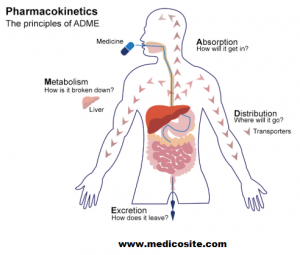
\includegraphics[width=0.6 \linewidth,height=0.5 \columnwidth]{/Users/yu-pinglin/Desktop/Essay/6001_LINGE.png}
    \centering
    \caption{The 4 pillars for building a sustainable portfolio of
    core facilities.}
\end{figure}
\section{CONCLUSION}
The exist of Pharmacokinetic studies will remaining a critical and unique role in the drug discovery process, to assist in the determination of effective and safe dosages of drug candidates, increasing the possibility of a candidate drug becoming an effective and safe therapy in man. 

\emergencystretch=1em
\printbibliography[title=Reference]

\end{document}




